\chapter{Modellierung}
\label{chap:SEVN}
\minitoc

Der durchschnittliche Energieverbrauch der Kälteanlagen je Supermaktkette
kann auf Grund der technischen Ausführung unterschiedlich sein. Der
Energieverbrauch entsteht an definierten Punkten im Netz. An den einzelnen
Knotenpunkten können mehrere Kältelasten angeschlossen sein.

%%%%%%%%%%%%%%%%%%%%%%%%%%%%%%%%%%%%%%%%%%%%%%%%%%%%%%%%%%%%%%%%%%%%%%%%%%%%%%%%
%%%%%%%%%%%%%%%%%%%%%%%%%%%%%%%%%%%%%%%%%%%%%%%%%%%%%%%%%%%%%%%%%%%%%%%%%%%%%%%%

\section{Erstellung des OOP-Modells}

In der \cref{vkb} wird ein einfaches Energieversorgungsnetz mit vier Knoten
dargestellt. Am Knoten eins ist eine regenerative elektrische Energiequelle, in
diesem Fall ein Windpark, angeschlossen. Weitere konventionelle elektrische
Energiequellen befinden sich an den Knoten zwei und drei. Die passiven Lasten
befinden sich am Knoten zwei und vier. Der Kältespeicher ist am Knoten zwei
angeschlossen. Im Bild wird der Kältespeicher Supermarkt durch einen
Einkaufswagen symbolisiert. Die Knoten sind untereinander durch Leitungen
verbunden.

\begin{figure}[h]
\caption{Vier Knoten Beispiel}
	\label{vkb}
	\begin{center}
	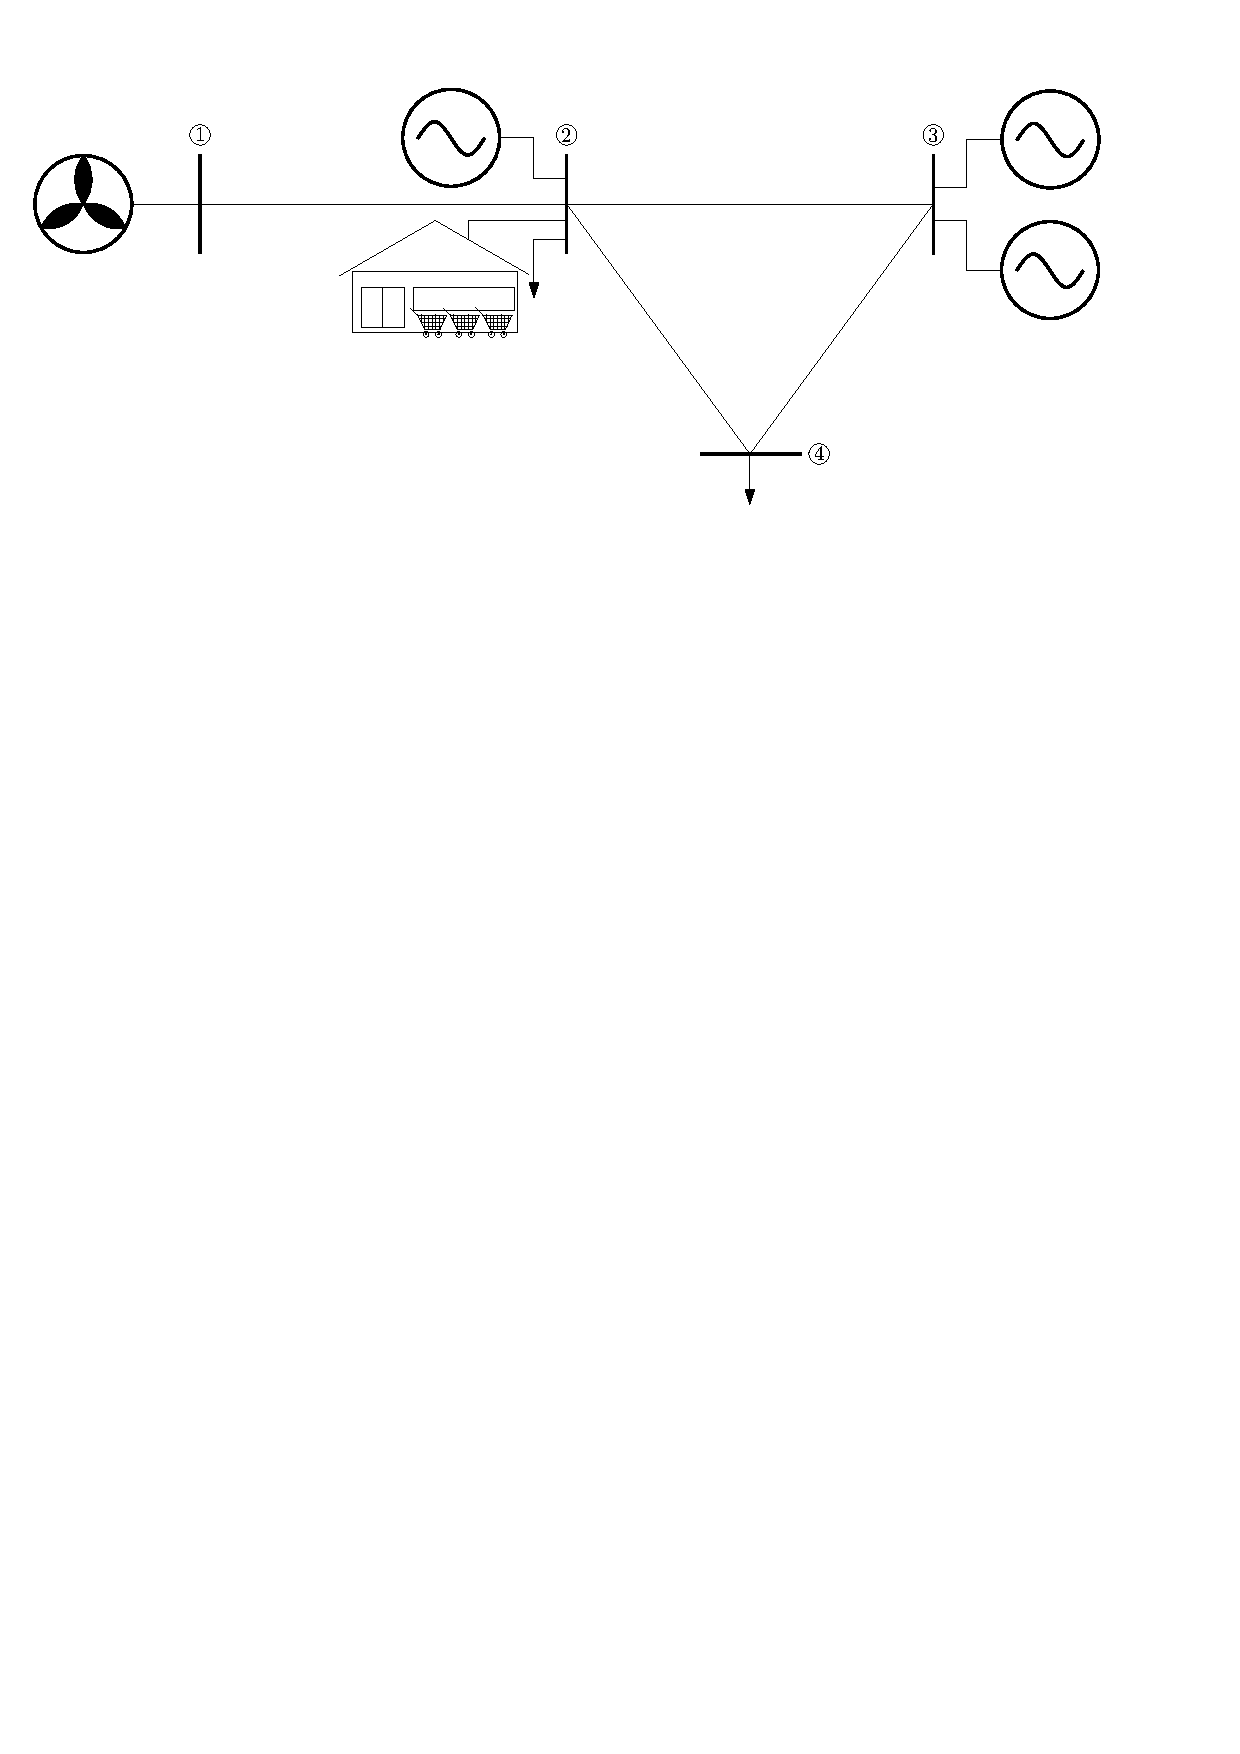
\includegraphics[scale=0.75]{images/SEVN/power_grid}
	\end{center}
\end{figure}



In der Realität kann ein Energieversorgungsnetz durch die Variation der
Knotenzahl und die Vermaschung beliebig komplizierte Form aufweisen. Bei der
Umsetzung der gegebenen Situation im Programm.

\begin{figure}[h]
\caption{Klassendiagramm Modellkonstrukt}
	\label{klassendiagramm}
	\begin{center}
	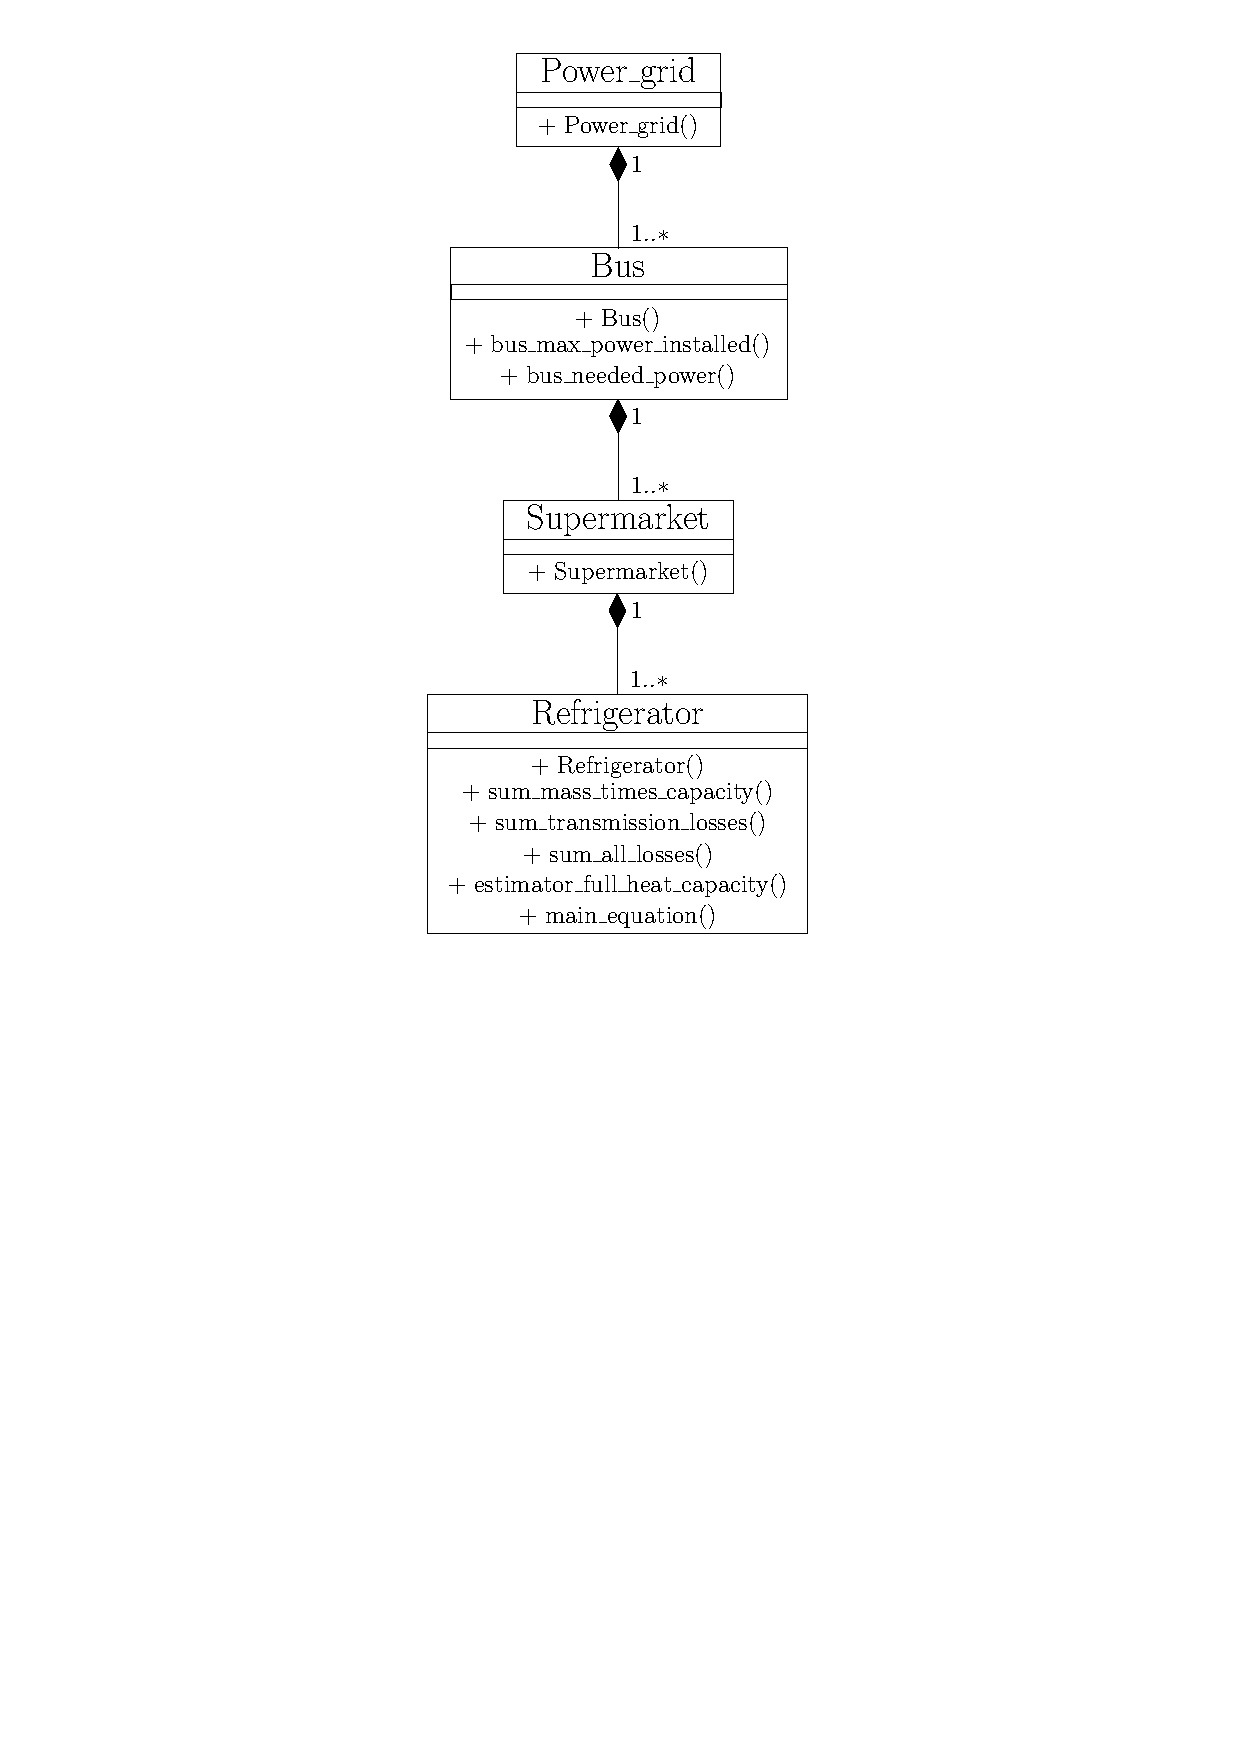
\includegraphics[scale=0.8]{images/Theorie_Super/class_diagramm}
	\end{center}
\end{figure}

Hier noch ein Zwischentext.

\begin{figure}[h]
\caption{Sequenzdiagramm Modellkonstrukt}
	\label{uml_sequence}
	\begin{center}
	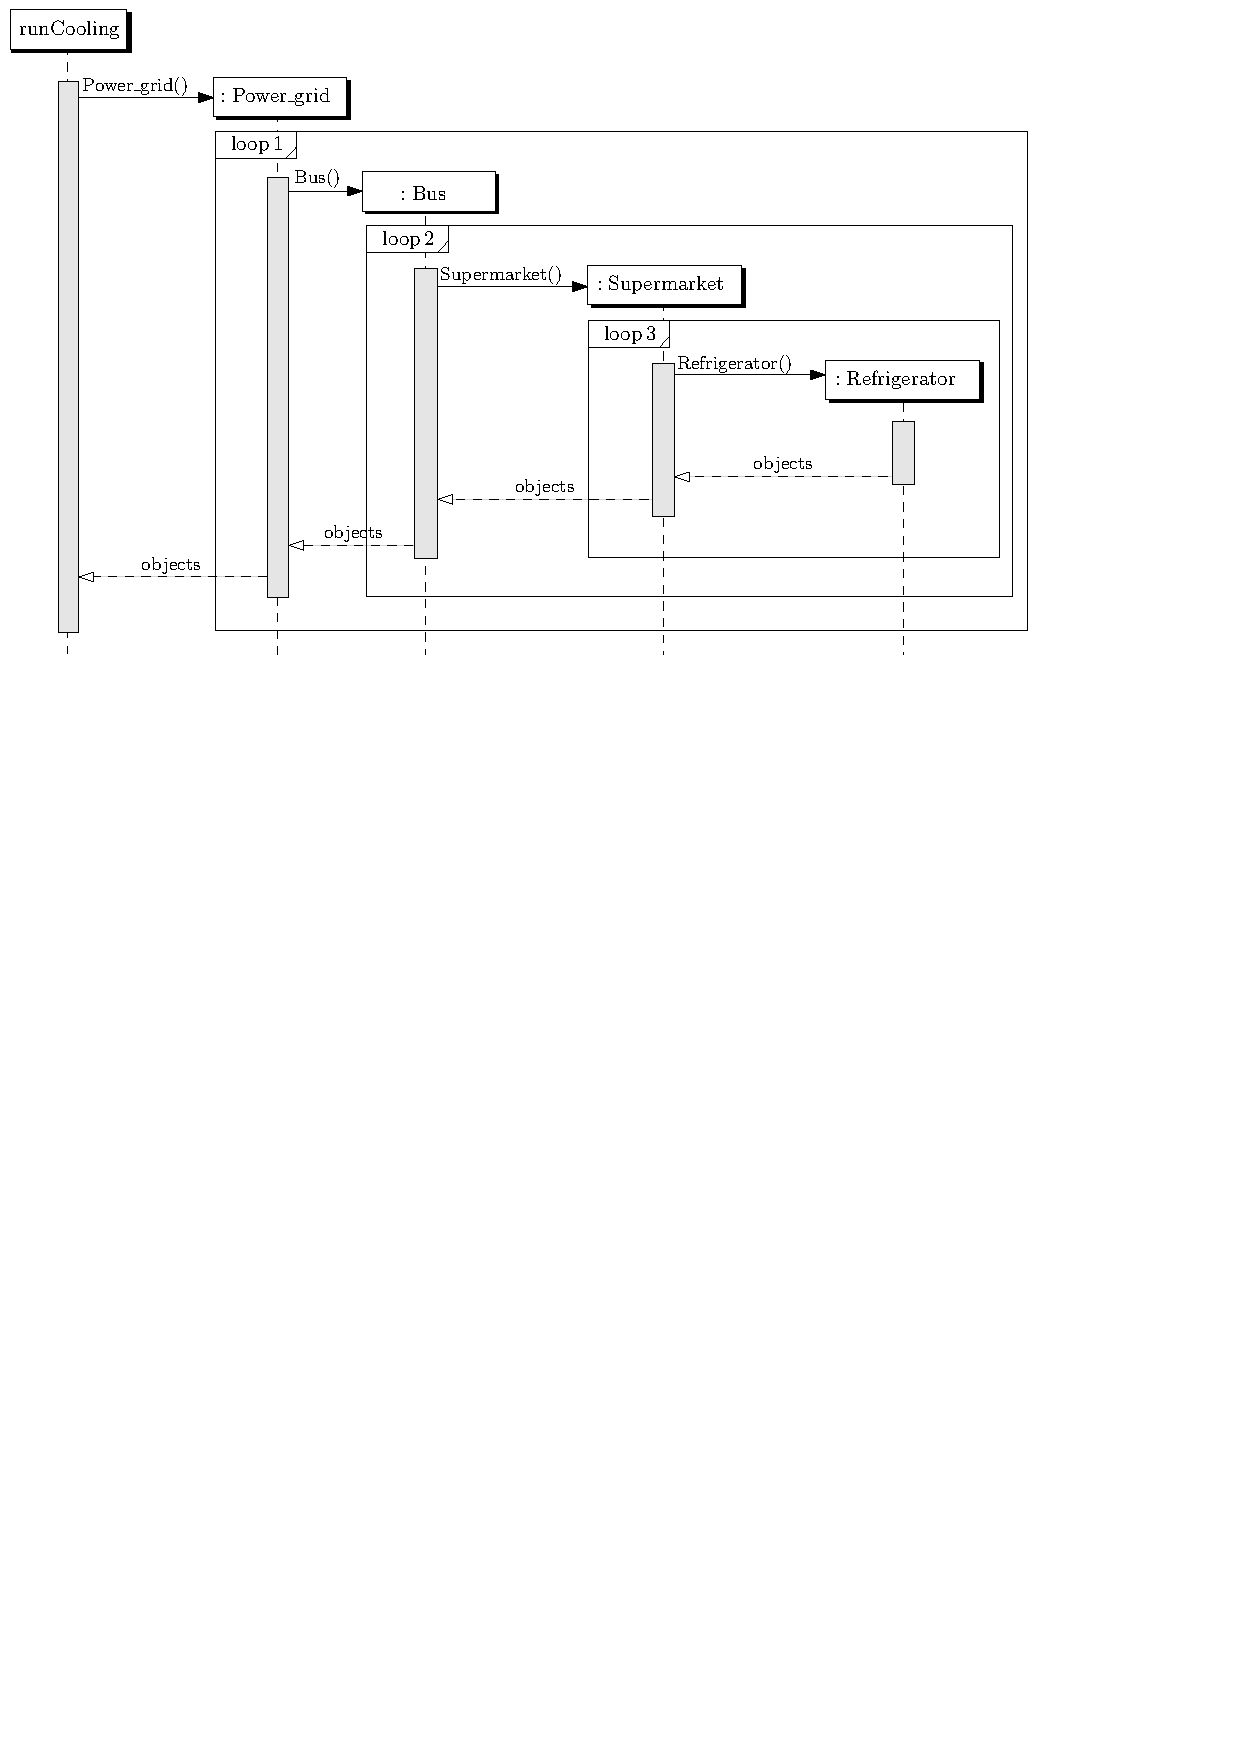
\includegraphics[scale=0.8]{images/Theorie_Super/sequence_one}
	\end{center}
\end{figure}

\section{Handhabung des Programms}
\label{sc:handhabung}

%%%%%%%%%%%%%%%%%%%%%%%%%%%%%%%%%%%%%%%%%%%%%%%%%%%%%%%%
%%%%%%%%%%%%%%%%%%%%%%%%%%%%%%%%%%%%%%%%%%%%%%%%%%%%%%%%
%%%%%%%%%%%%%%%%%%%%%%%%%%%%%%%%%%%%%%%%%%%%%%%%%%%%%%%%
\subsection{Allgemeines}

Das Programm ist ein Packet aus \matlab M-files zur Simulation von Kälteanlagen
mit Kältespeichern\footnote{ Da gewöhnliche Supermarktketten Untersuchungsobjekt
dieser Studie sind, werden die Termini Kältelast, Kälteanlagen mit
Kältespeichern und Supermarktkette als gleichbedeutend aufgefasst und
verwendet.} in einem Energieversorgungsnetz. Das Simulationsprogramm ist in der
Lage das Verhalten einer bzw. mehrerer Supermarktkälteanlagen als flexibler
Verbraucher in einem Energieversorgungsnetz zu simulieren. Das Programm kann
über eine vordefinierte Schnittstelle in ein Leistungsflussberechnungs-Programm
eingebunden werden.

%%%%%%%%%%%%%%%%%%%%%%%%%%%%%%%%%%%%%%%%%%%%%%%%%%%%%%%%
%%%%%%%%%%%%%%%%%%%%%%%%%%%%%%%%%%%%%%%%%%%%%%%%%%%%%%%%
%%%%%%%%%%%%%%%%%%%%%%%%%%%%%%%%%%%%%%%%%%%%%%%%%%%%%%%%
\subsubsection{Systemanforderungen}

Zur Benutzung des Programms muss auf Grund der gewählten Programmiersprache und
der objektorientierten Programmierwiese folgendes gelten:

\begin{itemize}
	\item Im Rechner muss die Software \matlab der Version $5.0$ oder
	höher\footnote{ \matlab verfügbar über The MathWorks, Inc.
	(http://www.mathworks.com).} eingerichtet sein.
\end{itemize}

Die Anforderungen an die Hardware sind durch die eingesetzte \matlab-Version
bestimmt.

%%%%%%%%%%%%%%%%%%%%%%%%%%%%%%%%%%%%%%%%%%%%%%%%%%%%%%%%
%%%%%%%%%%%%%%%%%%%%%%%%%%%%%%%%%%%%%%%%%%%%%%%%%%%%%%%%
%%%%%%%%%%%%%%%%%%%%%%%%%%%%%%%%%%%%%%%%%%%%%%%%%%%%%%%%
\subsubsection{Installation}

Das Programm richtet sich in seiner Installation und der Benutzung nach dem
allgemein gültigen Gebrauch der \matlab M-files\footnoteremember{matlab}{
	Ausführliche Information dazu findet man z.B. im \cite{MATLAB-Buch}.}.

%%%%%%%%%%%%%%%%%%%%%%%%%%%%%%%%%%%%%%%%%%%%%%%%%%%%%%%%
%%%%%%%%%%%%%%%%%%%%%%%%%%%%%%%%%%%%%%%%%%%%%%%%%%%%%%%%
%%%%%%%%%%%%%%%%%%%%%%%%%%%%%%%%%%%%%%%%%%%%%%%%%%%%%%%%
\subsubsection{Aufruf der Simulation}%

Die Primärfunktion des Programms ist, wie oben schon erwähnt, die Simulation des
Lastverhaltens eines Supermarkts oder mehreren Supermarktketten in einem
Energieversorgungsnetz. Das setzt voraus, dass folgende grundlegende Prinzipien
realisiert werden:
\begin{enumerate}
	\item Ein oder mehrere \matlab-Modelle von Supermärkten können erstellt
	und gleichzeitig an verschiedenen Knoten im Energieversorgungsnetz
	verwendet werden.
	\item Von einem besonderen Interesse sind die Energieverbrauchszahlen
	zum Beispiel für einen bestimmte Kälteeinheit oder für die gesamte
	Kette. Die Realisierung der Speicherung dieser Daten ist zwingend.
\end{enumerate}

%%%%%%%%%%%%%%%%%%%%%%%%%%%%%%%%%%%%%%%%%%%%%%%%%%%%%%%%
%%%%%%%%%%%%%%%%%%%%%%%%%%%%%%%%%%%%%%%%%%%%%%%%%%%%%%%%
%%%%%%%%%%%%%%%%%%%%%%%%%%%%%%%%%%%%%%%%%%%%%%%%%%%%%%%%
\subsubsection*{Vorbereitung der Input-Information}
\label{sec:input_infos}

Je nach Fall oder theoretischer Grundlage können die Konfigurationsdateien
verändert werden\todo{das ist scheiße!}.  Zum Starten des Programms werden
folgende Konfigurationsdateien benötigt:

\begin{itemize}
	\item config\_grid.m
	\item config\_supermarkets.m
	\item config\_fridges.m
\end{itemize}
%%%%%%%%%%%%%%%%%%%%%%%%%%%%%%%%%%%%%%%%%%%%%%%%%%%%%%%%
%%%%%%%%%%%%%%%%%%%%%%%%%%%%%%%%%%%%%%%%%%%%%%%%%%%%%%%%
%%%%%%%%%%%%%%%%%%%%%%%%%%%%%%%%%%%%%%%%%%%%%%%%%%%%%%%%
\vspace{3mm}
\noindent\textbf{config\_grid.m}
\vspace{3mm}

Es ist wichtig, dass die topologische Eigenschaft des Netzes im Programm
berücksichtigt werden, damit bei der Berechnung des Leistungsflusses die
Laständerung, die durch den Betrieb der Kältelast entsteht, am Knoten, an dem
sie verursacht wird, gezählt wird\todo{freaky sentence}. Damit das Programm mit
den für die Simulation notwendigen Informationen, die das Energienetz
beschreiben, versorgt wird, ist die Form, die in \matref{cgrid} vorgestellt
wird, für die \textbf{config\_grid.m$\,$}-Datei zwingend:

\begin{lstlisting}[float=h,caption={config\_grid.m},label={cgrid}]
%%	Bus,  Supermarkets,	  Number of Supermarkets
configuration_grid = {...
        1 , {Aldi	     ,	      1500;	     ...
             Netto	     ,	       500};	 ...
        2 , {0	         ,           0};	 ...
        3 , {0	         ,           0};	 ...
        4 , {0	         ,           0}	     ...
       };
\end{lstlisting}

In der \textbf{config\_grid.m}$\,$-Datei wird  ein $n\times2\,$-Cell Array
($n\in \mathbb{Z}^+_0$) definiert, der die Information über die Topologie des
Netzes sowie die Verteilung der Kältelasten im Netz beinhaltet. Ein Cell Array
ist ein Speicherobjekt, der verschiedene Datentypen unterschiedlicher Größe
aufnehmen kann\cite[Teil 2, Seite 15]{MATLAB-Buch}.  Ein Cell Array wird mit dem
Befehl $c=cell(\ldots)$ oder mit Hilfe von geschweiften Klammern $c=\{\ldots\}$,
wie in diesem Fall, erzeugt. Der Zugriff auf ein Cell Array wird in dem
folgenden Kapitel\todo{Hier auf Kapitel verweisen.}$\,$ kurz
erklärt\footnoterecall{matlab}. Jede Zeile des Cell Arrays
\textbf{configuration\_grid}, der in der \textbf{config\_grid.m}$\,$-Datei
definiert werden muss, steht für ein Knotenpunkt im Netz. In der ersten Spalte
wird die Nummer des Knotens bzw. Busses gespeichert. In die zweite Spalte werden
die Arten der Kältelasten und deren Anzahl an jeweiligen Knoten festgelegt. Es
ist wiederum ein $m\times2\,$-Cell Array ($m\in \mathbb{Z}^+_0$). Jede Zeile
dieses Cell Arrays ist für eine eigene Art Supermarktkette reserviert. In die
erste Spalte kommt der Name der Supermarktkette deren Eigenschaften in der
\textbf{config\_supermarkets.m$\,$}-Datei vergl.  \matref{csuper} gespeichert
sind. In die zweite Spalte wird die Anzahl der Supermärkte einer Kette
festgelegt die an dem bestimmten Knoten simuliert werden soll.

Um Fehler auf dieser Ebene zu vermeiden, muss die
\textbf{config\_grid.m}$\,$-Datei unbedingt die oben vorgestellte Form
beibehalten.

%%%%%%%%%%%%%%%%%%%%%%%%%%%%%%%%%%%%%%%%%%%%%%%%%%%%%%%%
%%%%%%%%%%%%%%%%%%%%%%%%%%%%%%%%%%%%%%%%%%%%%%%%%%%%%%%%
%%%%%%%%%%%%%%%%%%%%%%%%%%%%%%%%%%%%%%%%%%%%%%%%%%%%%%%%
\vspace{3mm}
\noindent\textbf{config\_supermarkets.m}
\vspace{3mm}

%%%%%%%%%%%%%%%%%%%%%%%%%%%%%%%%%%%%%%%%%%%%%%%%%%%%%%%%%%%%%%%%%%%%%%%%%%%%%%%%
% Abkürzungen die config_supermarkets betreffen
\abvz{NK\_KT\_S}{normalgekühlte Kühltruhe steckerfertig}
\abvz{NK\_KR\_V}{normalgekühltes Kühltregal an Verbundanlage}
\abvz{TK\_TKT\_S}{tiefgekühlte Tiefkühltruhe steckerfertig}
%%%%%%%%%%%%%%%%%%%%%%%%%%%%%%%%%%%%%%%%%%%%%%%%%%%%%%%%%%%%%%%%%%%%%%%%%%%%%%%%

\begin{lstlisting}[float=h!,caption=config\_supermarkets.m,label={csuper}]
%%       Kind of fridge
Aldi = {...
        NK_KT_S;     ...
        NK_KR_V;     ...
        TK_TKT_S     ...
       };
Netto = {...
        NK_KT_S      ...
       };
\end{lstlisting}

Die Kältelast in einem Supermarkt bilden die einzelnen je nach Einsatzzweck
speziell dafür konstruierten Kühleinheiten. Die Anzahl, die technischen
Eigenschaften und die Betriebsweise dieser Kältemaschinen können in der Realität
beispielsweise auf Grund von klimatischen, wirtschaftlichen oder auf
Kundenverhalten bezogenen Standortbesonderheiten Unterschiede
aufweisen\todo{Kältemaschinen beschreiben?}. Für eine breite Betrachtung des
Einflusses auf ein Energieversorgungsnetz durch den Einsatz unterschiedlicher
Supermaktketten ist es zweckmäßig die beschriebenen Besonderheiten im
Simulationsprogramm zu verfolgen. In der Konfigurationsdatei
\textbf{config\_supermarkets.m$\,$} (vergl. \matref{csuper}) wird festgelegt,
wie die einzelnen Supermarktketten aus verschiedenen Kälteeinheiten
zusammengesetzt sind. Die Gruppierung der einzelnen Kühleinheiten zu einem
Modellsupermarkt erfolgt in der \textbf{config\_supermarkets.m$\,$}-Datei durch
Definition eines oder mehrerer Cell Arrays, die jeweils ein Supermarkt abbilden.
Die Dimension eines solchen Arrays muss $i\times1\,$-Cell Array ($i\in
\mathbb{Z}^+_0$) sein\todo{$i\times1\,$eigentlich noch nicht ideal,
Schwachstelle, umdenken}. Jede Zeile eines solchen Cell Arrays ist für je eine
Art Kühleinheit reserviert. Die spezifischen Eigenschaften einer Kühleinheit
werden in der Konfigurationsdatei \textbf{config\_fridges.m} gespeichert.

%%%%%%%%%%%%%%%%%%%%%%%%%%%%%%%%%%%%%%%%%%%%%%%%%%%%%%%
%%%%%%%%%%%%%%%%%%%%%%%%%%%%%%%%%%%%%%%%%%%%%%%%%%%%%%%
%%%%%%%%%%%%%%%%%%%%%%%%%%%%%%%%%%%%%%%%%%%%%%%%%%%%%%%
\vspace{3mm}%
\noindent\textbf{config\_fridges.m}
\vspace{3mm}

Die Konfigurationsdatei \textbf{config\_fridges.m} kann als eine Datenbank für
Kälteeinheiten aufgefasst werden. In dieser Datenbank werden Informationen nach
einem bestimmten Muster gruppiert und gespeichert, sodass jede Gruppe eine
bestimmte Kühleinheit abbildet\todo{Beschränkungen hier?}. Im Programm kann aus
je einem dieser physikalisch fundierten Modellen\footnoteremember{carro}{ In
dieser Arbeit werden Kühleinheiten-Modelle verwendet, die von Caroline Möller in
ihrer Diplomarbeit \cite{caro} erarbeitet wurden.} ein Kühleinheit-Objekt
erzeugt werden. Abhängig von der Zusammensetzung der Konfigurationsdateien
\textbf{config\_grid.m} und \textbf{config\_supermarkets.m} wird die Zuweisung
im Gesamtmodell (Anzahl in einem bestimmten Supermarkt und an einen bestimmten
Knoten im Energieversorgungsnetz) durchgeführt.

Am Beispiel des Modells einer steckerfertigen
Normalkühltruhe\footnoterecall{carro}, abgekürzt NK\_KT\_S (vergl.
\matref{fridge}), wird im folgenden die Eingabeform eines solchen
Datenbankeintrages in der Datei \textbf{config\_fridges.m} erläutert. Zur
Beschreibung einer Kühleinheit ist erforderlich, die Daten in einen
$1\times15\,$-Cell Array zu erfassen.  Die Größe und die Art des Arrays ist
vorgegeben durch die im Modell getroffenen Annahmen\footnoterecall{carro} zur
Anzahl und dem Typus der modellbeschreibenden Daten. Die Struktur eines Cell
Arrays ermöglicht neben der zusammenhängenden Speicherung verschiedener
Datentypen einen durch \matlab darauf direkten Zugriff.

\begin{lstlisting}[caption=config\_fridges.m,label={fridge}]
1  % fridge configuration parameters
2  NK_KT_S = { ...
3          1, ... % 1 if plugin module or 2 if combine fridge
4          4.7e3, ... % energy consumption per day Wh/24h
5          2, ... % epsilon power quotient
6          0.66, ... % compressor quotient
7          0 ... % installed cooling power in W
8          2, ... % number_of_walls
9          [16.4 6.7], ... % area_wall
10         [0.38 0.38], ... % heat_transmission_coefficient
11         [19 15], ... % temperature_outside
12         [200 200], ... % masse_stored
13         [2.3 3.52], ... % specific_mass_capacity
14         -6, ... % temperature_min in Celsius
15         2, ... % temperature_max in Celsius
16         1, ... % averaged cooling room temperature in Celsius
17         0, ... % refrigerating capacity
18        };
\end{lstlisting}

\begin{description}

	\item [{Spalte eins}] (vergl. Zeile 3 im \matref{fridge}\todo{das ist
	doch überflüssig, oder?}) Die Unterscheidung in steckerfertige
	Kälteanlagen und Kälteverbundanlagen im Programm ist notwendig, da bei
	der Berechnung der Kälteverluste unterschiedliche Verfahren zu Grunde
	gelegt werden\todo{Das ist noch zu Überprüfen}.  Diese Differenzierung
	erfolgt durch die Zuweisung einer Eins für die steckerfertige Einheit
	und einer Zwei für eine Einheit an Verbundanlage in der ersten Spalte im
	Array .

	\item [{Spalte zwei}] Die druchschnittliche elektrische Energieaufnahme
	ist eine Kennzahl in Watt pro 24 Stunden, die durch die Hersteller mit
	Hilfe eines genormten Verfahren ermittelt wird und in den technischen
	Blättern angegeben werden muss\todo{Wo wird das Verwendet? Hier
	schreiben}.

	\item [{Spalte drei}] In diese Spalte wird die Leistungszahl
	(ausführlich beschrieben im \cref{Leistungszahl}) eingetragen.

	\item [{Spalte vier}] Der Anteil des Verdichters an dem
	Tagesenergieverbrauch der Kühleinheiten wird Leistungszahl genannt. Aus
	der \cref{lverd} im \cref{chap:theorie} geht hervor, wie diese Kehnzahl
	in die Berechnung eingeht. Die Liestungszahl wird in der Spalte vier
	festgehalten.

	\item [{Spalte fünf}] Werden anschlussfertige Kälteaggrigate zur Kühlung
	von Räumen verwendet, so wird die installierte Kälteleistung in Kilowatt
	in die Spalte fünf anstatt einer Null eingetragen.

	\item [{Spalte sechs}] Ein Teil der Wärmeverluste ist auf die
	Transmissionsverluste durch die Wände zurückzuführen.  Die Anzahl der
	Wände muss für die Rechnung berücksichtigt werden, Sie wird in die
	sechste Spalte eingetragen.
	
	\item [{Spalte sieben}] Für die Transmissionsverlustberechnung sind
	under anderen die Flächengrößen und die jeweiligen
	Wärmedurchgangskoeffizienten der einzelnen Wände
	maßgebend\footnoteremember{Waende}{ Der mathematische Zusammenhang wird
	im \cref{chap:theorie} in der \cref{ptrans} deutlich gemacht.}. Für je
	eine Flächengröße in Quadratmeter ist in der Spalte sieben des
	NK\_KT\_S-Arrays ein Spaltenplatz im $1\times w\,$-Zeilenarray
	reserviert. Die $w$ steht für die Anzahl der Wände.

	\item [{Spalte acht}] In der achten Spalte werden in einem weiteren
	$1\times w\,$-Zeilenarray die mit den Flächen korrespondiere
	Wärmedurchgangskoeffiziente\footnoterecall{Waende} in gleicher
	Reihenfolge gespeichert.

	\item [{Spalte neun}] Die Tepmeratur außerhalb der Kühleinheit
	bestimmt\footnoterecall{Waende} die Größe der Transmissionsverluste. In
	der neunten Spalte werden nach dem gleichen Prinzip und in der gleichen
	Form wie im vorhergegangenen Eintrag die Außentemperatur für jede Wand
	eingetragen.

	\item [{Spalte zehn}] Die Abhängigkeit der Temperaturänderung von der in
	einer Kühleinheit deponierten Masse an Waren und deren spezifische
	Wärmekapazität ist aus der \cref{tdif} im \cref{chap:theorie}
	ersichtlich. In der Realität werden in einem Kühlschrank gewöhnlich
	mehrere verschiedene Lebensmittel gekühlt. Möchte man gemischte Beladung
	simulieren, so sind die Massen in der Spalte zehn im NK\_KT\_S in der
	gleichen Art und Weise wie in der Spalte sieben acht oder neun zu
	einzutragen. Der Eintrag erfolgt in Kilogramm.

	\item [{Spalte elf}] Zu jeder in der Spalte zehn eingetragener Massezahl
	muss in der Spalte neun nach dem Beispiel der Spalte acht die
	spezifische Wärmekapazität eingetragen werden.

	\item [{Spalte zwölf}] In der Realität fällt die Spanne für Variation
	die Innentemperatur in einem Lebensmittelkühlschrank eher gering aus, da
	die Temperatur auf einem bestimmten Niveau gehalten werden muss, damit
	die Lebensmittel maximal lange frisch bleiben können. Möchte man die
	Kälte im Lebensmittel speichern, darf die Lebensmitteltemperatur einen
	bestimmten Bereich nicht Verlassen. In der Spalte zwölf im NK\_KT\_S
	wird die untere Temperaturgrenze in Grad Celsius festgelegt.

	\item [{Spalte elf}] In der Spalte elf wird die obere Temperaturgrenze
	in Grad Celsius festgelegt.

	\item [{Spalte zwölf}] Die Bedeutung\footnoteremember{v:caro}{
	Ausführlich begründet wird das in \cite{caro}.} der mittleren
	Kühlraumtemperatur ist kurz im \cref{chap:theorie} angeschnitten.
	Notiert wird diese Kennzahl in der Spalte zwölf im NK\_KT\_S
	eingetragen.

	\item [{Spalte dreizehn}] Keine Ahnung\todo{Klären was das ist.}

\end{description}
%%%%%%%%%%%%%%%%%%%%%%%%%%%%%%%%%%%%%%%%%%%%%%%%%%%%%%%%
%%%%%%%%%%%%%%%%%%%%%%%%%%%%%%%%%%%%%%%%%%%%%%%%%%%%%%%%
%%%%%%%%%%%%%%%%%%%%%%%%%%%%%%%%%%%%%%%%%%%%%%%%%%%%%%%%
\subsubsection*{Die main.m Datei}
%%%%%%%%%%%%%%%%%%%%%%%%%%%%%%%%%%%%%%%%%%%%%%%%%%%%%%%%
%%%%%%%%%%%%%%%%%%%%%%%%%%%%%%%%%%%%%%%%%%%%%%%%%%%%%%%%
%%%%%%%%%%%%%%%%%%%%%%%%%%%%%%%%%%%%%%%%%%%%%%%%%%%%%%%%
\subsubsection{Deklamation der berechneten Daten}
%%%%%%%%%%%%%%%%%%%%%%%%%%%%%%%%%%%%%%%%%%%%%%%%%%%%%%%%
%%%%%%%%%%%%%%%%%%%%%%%%%%%%%%%%%%%%%%%%%%%%%%%%%%%%%%%%
%%%%%%%%%%%%%%%%%%%%%%%%%%%%%%%%%%%%%%%%%%%%%%%%%%%%%%%%

Die inhaltliche Auswertung der Simulation ist dem Benutzer vorbehalten. Darum
müssen die Ergebnisse der Simulation in einer anwenderfreundlichen Form
zugänglich gemacht werden. Durch sinnvolle graphische Darstellung der
untersuchten Größen kann zum Beispiel die Überprüfung, die Veranschaulichung
oder die Bestimmung der funktionalen Abhängigkeit dieser durchgeführt werden.
\todo[inline,color=orange!30]{Das ist noch nicht richtig im Programm
implementiert. Das muss DU NOCH MACHEN!}


%%%%%%%%%%%%%%%%%%%%%%%%%%%%%%%%%%%%%%%%%%%%%%%%%%%%%%%%
%%%%%%%%%%%%%%%%%%%%%%%%%%%%%%%%%%%%%%%%%%%%%%%%%%%%%%%%
%%%%%%%%%%%%%%%%%%%%%%%%%%%%%%%%%%%%%%%%%%%%%%%%%%%%%%%%
\subsubsection*{Graphische Ausgabe}
\textbf{Wichtig!!!} hier wird nicht der Quellcode erklärt, sondern die
Darstellung der Ausgabe.  \todo[inline,color=orange!30]{Funktion mit für die
graphische Ausgabe schreiben}
\subsubsection{Tabellarische Ausgabe im Command-Window und Exel}
\todo[inline,color=orange!30]{Funktion für tabellarische Ausgabe schreiben}

